\section{Durchführung}
\begin{figure}
    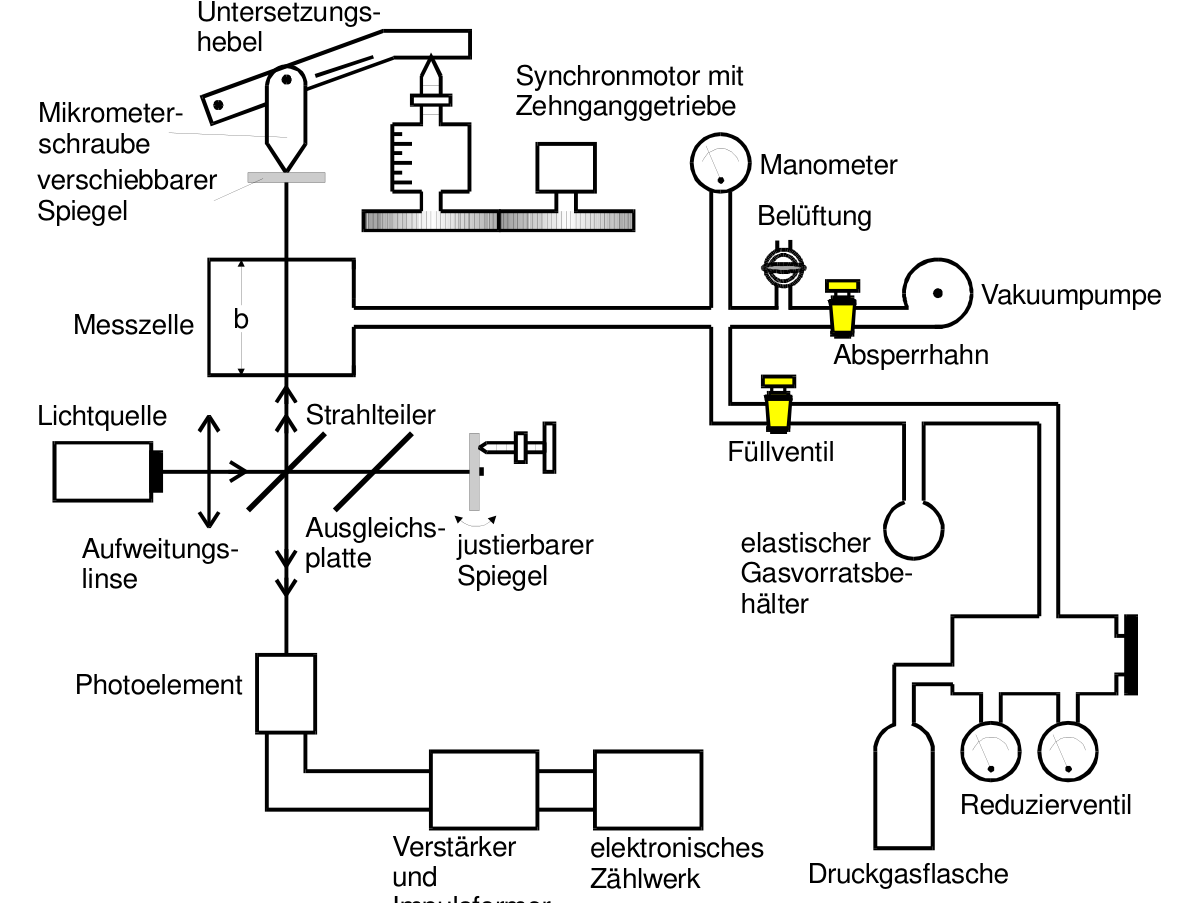
\includegraphics[width=\textwidth]{Abbildungen/Screenshot (5).png}
    \caption{Schematischer Versuchsaufbau.}
    \label{fig:Aufbau}
\end{figure}
Das hier verwendete Michelson-Interferometer ist in Abbildung \ref{fig:Aufbau} zu sehen.
Für eine lange Kohärenzlänge wird als Lichtquelle eine LASER-Diode mit einer Wellenlänge von \textbf{Wellenlänge einfügen} verwendet. 
Zunächst der justierbare Spiegel am Ende des einen optischen Armes eingestellt um die hellsten Lichtpunkte auf dem Photoelement zusammenzubringen.

In dem Photoelement wird die Lichtintensität des zusammengeführten Lichtes gemessen.
Intensitätsimpulse werden von einem Verstärker rechteckmäßig Transformiert und anschließend von einem Impulszähler gezählt.
% Hier werden sich die Interferenzphänomene zunutze gemacht, die im Folgenden 
Für die Messung der Wellenlänge wird ein Spiegel mit einem Synchrotron Motor langsam in Richtung des Lasers bewegt.
An der Mikrometerschraube wird die Auslenkung $\Delta d$ der Schraube zwischen \qty{4}{\mm} und \qty{9}{\mm} eingestellt.
Diese Messung wird 10 mal wiederholt und die Impulsanzahl wird notiert

Für die Messung des Brechungsindex der Luft wird die Messkammer der Tiefe $b = \qty{50}{\mm}$ mit einer Handpumpe auf \qty{600}{\mmHg} evakuiert 
und anschließend die Luft wieder reingelassen. Für beide Prozesse wird die Impulsanzahl notiert.